s
\documentclass{article}

% if you need to pass options to natbib, use, e.g.:
% \PassOptionsToPackage{numbers, compress}{natbib}
% before loading nips_2017
%
% to avoid loading the natbib package, add option nonatbib:
% \usepackage[nonatbib]{nips_2017}

\usepackage{nips_2017}

% to compile a camera-ready version, add the [final] option, e.g.:
% \usepackage[final]{nips_2017}

\usepackage[utf8]{inputenc} % allow utf-8 input
\usepackage[T1]{fontenc}    % use 8-bit T1 fonts
\usepackage{hyperref}       % hyperlinks
\usepackage{url}            % simple URL typesetting
\usepackage{booktabs}       % professional-quality tables
\usepackage{amsfonts}       % blackboard math symbols
\usepackage{nicefrac}       % compact symbols for 1/2, etc.
\usepackage{microtype}      % microtypography
\usepackage[utf8]{inputenc} % allow utf-8 input
\usepackage[T1]{fontenc}    % use 8-bit T1 fonts
\usepackage{hyperref}       % hyperlinks
\usepackage{url}            % simple URL typesetting
\usepackage{booktabs}       % professional-quality tables
\usepackage{amsfonts,amsthm}       % blackboard math symbols
\usepackage{nicefrac}       % compact symbols for 1/2, etc.
\usepackage{microtype}      % microtypography
\usepackage{MnSymbol}
\usepackage{color}
\usepackage{graphicx} % more modern
\usepackage{subfigure} 
\usepackage{natbib}
\usepackage{algorithm}
\usepackage{algpseudocode}
\usepackage{lineno}
\usepackage{thmtools,thm-restate}
\usepackage{xr}

%\linenumbers



\def\A{\mathcal{A}}
\def\ga{\gamma_\mathcal{A}}
\def\Co{C^{\circ}}
\def\Coa{C^{\circ}_{\!\!\mathcal{A}}}
\def\Ca{C_{\!\mathcal{A}}}
\def\go{\gamma^{\circ}}
\def\goa{\gamma^{\circ}_{\A}}
\newcommand{\dt}[2]{\langle#1,#2\rangle}
\def\Olasso{\Omega_{\rm Lasso}} % Lasso norm
\def\Ogl{\Omega_{\rm GL}} % group Lasso norm
\def\Olgl{\Omega_{\rm LGL}} % latent group Lasso norm
\def\tr{{\rm tr}}
\newcommand\itgset[1]{[\!\![#1]\!\!]}
\def\RR{\mathbb{R}}
\def\EE{\mathbb{E}}
\newcommand{\tblue}[1]{\textcolor{blue}{#1}}
\newcommand{\tred}[1]{\textcolor{red}{#1}}
\newcommand\TODO[1]{\tblue{TODO: \texttt{#1}}}
%\newcommand\TODO[1]{}
\newcommand\OLD[1]{\tblue{#1}}
\newcommand\NEW[1]{\tred{#1}}
\def\st{\text{s.t.}}
\def\supp{\text{supp}}

\def\BIT{\begin{itemize}}
\def\EIT{\end{itemize}}
\def\BET{\begin{enumerate}}
\def\EET{\end{enumerate}}
\def\ra{$\:\rightarrow\:$}
\def\y{\mathbf{y}}
\def\x{\mathbf{x}}
\def\v{\mathbf{v}}
\def\u{\mathbf{u}}
\def\w{\mathbf{w}}
\def\s{\mathbf{s}}
\def\g{\mathbf{g}}
\def\h{\mathbf{h}}
\def\X{\mathbf{X}}
\def\RR{\mathbb{R}}
\def\ei{\varepsilon_i}
\def\ej{\varepsilon_j}
\def\T{\mathcal{T}}
\def\I{\mathcal{I}}

\def\op{{\rm op}}
\def\supp{{\rm Supp}}
\def\st{\text{s.t.}}
\newcommand\normop[1]{|||#1|||_{\infty}}
\newcommand\normbop[1]{|\!|\!|#1|\!|\!|_{\infty,2}}
\newcommand\normopop[1]{|\!|\!|#1|\!|\!|_{\rm op,\rm op}}
\newcommand\ve[1]{\varepsilon^{{\scriptscriptstyle#1}}}
\newcommand\sss[1]{{\scriptscriptstyle#1}}
\def\uI{U^{\sss{I}}}
\def\xxi{\zeta}

\newtheorem{thm}{Theorem}
\newtheorem{prop}{Proposition}
\newtheorem{fact}{Fact}
\newtheorem{lemm}{Lemma}
\newtheorem{coro}{Corollary}
\newtheorem{mydef}{Definition}

\title{Learning the effect of latent variables in Gaussian Graphical models with unobserved variables}

% The \author macro works with any number of authors. There are two
% commands used to separate the names and addresses of multiple
% authors: \And and \AND.
%
% Using \And between authors leaves it to LaTeX to determine where to
% break the lines. Using \AND forces a line break at that point. So,
% if LaTeX puts 3 of 4 authors names on the first line, and the last
% on the second line, try using \AND instead of \And before the third
% author name.

\author{
  David S.~Hippocampus\thanks{Use footnote for providing further
    information about author (webpage, alternative
    address)---\emph{not} for acknowledging funding agencies.} \\
  Department of Computer Science\\
  Cranberry-Lemon University\\
  Pittsburgh, PA 15213 \\
  \texttt{hippo@cs.cranberry-lemon.edu} \\
  %% examples of more authors
  %% \And
  %% Coauthor \\
  %% Affiliation \\
  %% Address \\
  %% \texttt{email} \\
  %% \AND
  %% Coauthor \\
  %% Affiliation \\
  %% Address \\
  %% \texttt{email} \\
  %% \And
  %% Coauthor \\
  %% Affiliation \\
  %% Address \\
  %% \texttt{email} \\
  %% \And
  %% Coauthor \\
  %% Affiliation \\
  %% Address \\
  %% \texttt{email} \\
}

\begin{document}
% \nipsfinalcopy is no longer used

\maketitle

\begin{abstract}
Gaussian graphical models (GGM) have been widely used in many high-dimensional applications. Some effects can affect the data, that is, some of the relevant variables may be latent. In this paper, we focus on a family of Latent Variable Gaussian graphical models (LVGGM), where the model is conditionally sparse given latent variables, but marginally non-sparse. In order to identify the effect of each latent variable and recover the structure of the complete model, we introduce a convex formulation with a new regularization imposing more structure on latent factors.  We propose a tractable convex algorithm and study identifiability conditions. We show promising results on synthetic and real datasets.\\
\end{abstract}



\section{INTRODUCTION}
\label{intro}


Graphical models have emerged as useful tools for modelling complex systems. In many fields such as genomics and finance among others, we have to analyze high-dimensional data, where the number of variables is of the same order or larger than the number of samples.  High-dimensional setting leads to ill-conditioned problems where some form of regularization needs to be imposed.

In the context of Gaussian Graphical Models (GGM), a central problem is to estimate the inverse covariance matrix, also known as the precision or concentration matrix. The sparsity pattern of the concentration matrix in such models corresponds to the structure of the graph, i.e. the nonzeros of the concentration matrix correspond to the edges of the graphical model. The model selection method usually studied in such a GGM setting is the graphical Lasso $\ell_1$-regularized maximum-likelihood \citep{friedman2008sparse,yuan2007model,banerjee2008model}.

Applications in which all relevant variables have been identified and measured are extremely rare. Some of the relevant variables may be latent inducing correlations between observed variables that can be misleading and can only be explained correctly if the presence of latent variables is explicitly modelled. More precisely, when latent variables are missing, the marginalized precision matrix may not be sparse even if the full precision matrix is sparse. Imposing sparsity on the complete model results on a marginal precision matrix of the Latent Variable Gaussian Graphical Model (LVGGM) that has a sparse plus low-rank structure. \citet{chandrasekaran2010} consider a regularized maximum likelihood approach, using $\ell_1$-norm to recover the sparse component and trace norm to recover the low-rank component and show that they consistently estimate the sparsity pattern of the sparse component and the number of latent variables. Their method identifies the low-rank structure corresponding to the effect of latent variables but it does not allow us to identify the covariance structure of each latent variable individually and it does not identify which observed variables are directly dependent of the unobserved ones and so which observed variables are conditionally independent of the latent variables given the others.


%With the obtained decomposition one identifies the structure of the conditional graphical model on the observed variables and the subspace of latent variables. However the decomposition fails to identify the effect of each latent variable separately since the subspace of latent variables does not have a unique decomposition. Choosing the orthogonal decomposition (SVD) gives us one choice. In our setup we want to impose some additional structure to the low-rank component in order to be able to identify the complete LVGGM structure.  

\citet{richard2014tight} introduce a new matrix norm that, when used as a regularizer, leads to  estimates for low-rank matrices with multiple sparse factors that are provably more efficient statistically than the $\ell_1$ and trace norms.

In this work, we propose to impose more structure on the low rank matrix using a generalization of the trace norm introduced in \citet{richard2014tight} as a regularizer. The obtained decomposition gives the structure of the complete graphical model and provides better interpretability of the graphical model. We propose a convex formulation with a quadratic loss function that can be optimized efficiently with the algorithm proposed in \citet{vinyes2017}.  Finally we study the identifiability of such decomposition. 

The paper is structured as follows. In Section \ref{related} we review the relevant prior literature. In Section {setup} we formulate the LVGGM estimation problem as a regularized convex problem that imposes a sparsity structure on the latent variables, we also propose a tractable algorithm. In Section \ref{sec:id} we study identifiability conditions. Experimental results are shown in Section \ref{experiments}.

\subsection*{Notations}
$\itgset{p}$ denotes the set $\{1,...,p\}$ and $\mathcal{G}^p_k$ denotes the
set of subsets of $k$ elements in $\itgset{p}$. $|I|$ denotes the cardinality of a set $I$. If $v\in\RR^{p}$ is a vector, $\supp(v)$ denotes its support. If $M\in\RR^{p\times p}$ is a matrix, $I\subset\itgset{n}$ , $M_{II}\in\RR^{|I|\times |I|}$ is the submatrix obtained by selecting the rows and columns indexed by $I$ in $M$. For a symmetric matrix $M$, $\lambda_{\max}^+(M)$ is the largest positive eigenvalue and zero if they are all negative.

%In many applications as genetics, finance...learning structure of graphical models. with more interpretability and more efficient inference if sparse. (cf drton for application examples). Speciffically, if the number of variables is very large compared to the number of samples
%We focus on learning undirected gaussian graphical models. A well studied problem is model selection where the inverse of the covariance, also called concentration matrix, is sparse. The nonzeros of the concentration matrix correspond to the edges of the graphical model. Graphical Lasso is the method of choice.
%Here model selection problem with latent variables. In applications where latent variables are missing, this may create non sparsity for some components on the graph, fully connecting all the observed variables connected to the latent variable, see Figure. 
%Why learning GGM, then latent GGM to learn models with more interpretability and more efficient inference if sparse. With no a priori on the number of latent variables.
%An interesting idea is to add sparsity to latent components. Theory on decomposition, more difficult if sparse latent components. 
%
%figure latent graphical model
 
\section{Related Work}
\label{related}
GGM l1\\
. Yuan and Lin (2007) and Banerjee et al. (2008) proposed the graphical lasso (glasso) estimator
A conditional independence graph is sometimes expected to have particular structure, such as ‘hub’ nodes with many neighbors. This motivated Defazio and Caetano (2012) to consider
regularization with a sorted ?1 norm.
GGM with other regularizations\\
LGGM\\
\citet{hosseini2016learning}
\citet{chandrasekaran2010}

ref in hosseini
\citet{tan2015cluster}
\citet{marlin2009sparse}
\citet{celik2014efficient}

\section{Problem setup}
\label{setup}

\subsection{Latent Variable GGM}
\label{sec:ggm}
We consider a multivariate Gaussian variable $(X_{O},X_{H})\in\RR^{p+h}$ where $O$ and $H$ are the set of indices of observed variables, $p=|O|$, and latent variables, $h=|H|$ respectively. We denote $\Sigma\in\RR^{(p+h)\times(p+h)}$ the complete covariance matrix and $K=\Sigma^{-1}$ the complete concentration matrix. Let $\hat{\Sigma}\in\RR^{(p+h)\times(p+h)}$ denote the empirical covariance matrix. We only have access to the empirical marginal covariance matrix $\hat{\Sigma}_{OO}$. It is well known that the marginal concentration matrix on the observed variables can be computed from the full concentration matrix as

\begin{align}
\Sigma_{OO}^{-1} = K_{OO}-K_{OH}K_{HH}^{-1}K_{HO}.
\end{align}

We assume that the original graphical model is sparse and that there is a small number of latent variables. In GGMs, the sparsity pattern of the concentration matrix  directly corresponds to the graphical model structure. This implies that  $K$ is a sparse  and therefore $K_{OO}$ is a sparse matrix. Having a small number of latent variables gives that $K_{OH}K_{HH}^{-1}K_{HO}$ is low-rank. Since $K$ is a concentration matrix, it is positive semidefinite (p.s.d.), which results in  $K_{OO}$ and $K_{OH}K_{HH}^{-1}K_{HO}$ being p.s.d.. $\Sigma_{OO}^{-1}$ is also p.s.d. as it is also a concentration matrix. \citet{chandrasekaran2010} suggest to approximate $\hat{\Sigma}$  by $S-L$ where $S$ is sparse and $L$ is low rank, where $S-L$, $S$ and $L$ are p.s.d. and propose propose a convex relaxation 
%Specifically, the nonzeros of the concentration matrix correspond to the edges of the graphical model. 
%The sparsity of the complete GGM implies that $K$ is sparse. Then, $K_{OO}$ should be a sparse matrix and assuming has a small number of latent variables is low rank. \citet{chandrasekaran2010} suggest to approximate $\hat{\Sigma}$  by $S-L$ where $S$ is sparse and $L$ is low rank, and propose a convex relaxation

\begin{align}
\label{opt_tr}
\min_{S,L} f(S-L)+\lambda\left(\gamma\|S\|_{1}+ \tr(L)\right) \quad s.t. \quad S-L \succeq 0 \quad L \succeq 0,
\end{align}

where the function $f$ is the loss function and the positivity constraint on $S$ has been dropped since it is implied by $S-L \succeq 0$ and $L \succeq 0$. Typically, in GGM seletion $f$ is the negative log-likelihood

\begin{align}
f_{ML}(M)&:=-\log\det(M) + \tr(M\hat{\Sigma}).
\end{align}

% LATER However $\textit{logdet}$ is not smooth\footnote{does not have Lipschitz gradients} preventing us from applying efficient algorithms from the family of conditional gradient, for which there is not convergence results for this setting.
 
Two other natural losses, that have the advantage of being quadratic, are the second order Taylor expansion arount the identity matrix of the log-likelihood $f_{T}$ and the score matching loss $f_{SM}$, introduced by \citet{hyvarinen2005estimation} and used for GGM estimation in \citet{lin2016estimation},
\begin{align}
f_{T}(M)&:=\frac{1}{2}\|\hat{\Sigma}^{1/2}M\hat{\Sigma}^{1/2}-I\|_2^2\\
f_{SM}(M)&:=\frac{1}{2}\tr(M^2 \hat{\Sigma})-\tr(M).
\end{align}

\citet{chandrasekaran2010} show that under appropriate tecnical conditions, the regularized maximum log-likelihood formulation (\ref{opt_tr}) provides estimates  that have the same sparsity pattern and rank than $K_{OO}$ and $K_{OH}K_{HH}^{-1}K_{HO}$. The obtained low rank component of the estimates retrieves the latent variable subspace. However it does not recover its structure, in particular the connectivity between the variables $(X_{O}$ and $X_{H})$ cannot be recoverd since ther is not a unique decomposition of the low rank component.\\

\TODO{explain better}
The low rank component writes $UU^{\top}$, where $U\in\RR^{p\times h}$. If we assume that the latent variables are independent, i.e. $K_{HH}$ is  diagonal,  unicity of the decomposition $UU^{\top}$ can be achieved by imposing more structure on the low rank component, which we discuss in the next paragraph \ref{subsec:norm}. Under appropriate identifiability conditions, discussed in section \ref{sec:id}, it allows us to retrieve the structure of the full LVGGM. In order to obtain a convex formulation we introduce a norm for low rank \textit{positive semidefinite} (p.s.d.) matrices with multiple sparse factors. 

%and that the decomposition is unique (see section \ref{sec:id} on identifiability).  Unicity of $K_{OH}$ is achieved imposing more structure on the low rank component, which we discuss in the next paragraph.
 
%talk here about structure of $K_{OO}-K_{OH}K_{HH}^{-1}K_{HO}.$  structure $S-L$ explain\\

%and three losses ML and the two quadratic\\

%$UU$ decomposition with sparsity on columns... Transition, in order to obtain convex formulation..\\
%
%\begin{align}
%FIGURE ?
%\end{align}

\TODO{transition}

\subsection{Positive-rank($k$) and its relaxation}
\label{subsec:norm}

\citet{richard2014tight} propose a new matrix norm that yields estimates for low-rank matrices with multiple sparse factors. In particular, these authors define a norm for p.s.d. matrices \footnote{In fact it is a gauge. For more on gauges see \citet{chandrasekaran2010convex} and references therein.}  that yields to estimates with sparse and p.s.d factors. In this sectionreview the concepts introduced by \citet{richard2014tight} and introduce the positive-rank($k$). We assume that the sparsity of the factors is known and fixed and discuss a generalization for factors of different sparsity levels at the end of the section.

The following definition generalizes the notion of rank for p.s.d matrices,
\begin{mydef}
(positive-rank($k$)) For a p.s.d  matrix $Z\in\RR^{p\times p}$ and for $k>1$ we define its positive-rank($k$) as the optimal
value of the optimization problem:
\begin{align}
\min \|c\|_0 \quad \text{s.t.} \quad Z=\sum_{i} c_i u_i u_{i}^\top, \quad c_i\in \RR^{+} \quad u_{i}\in\RR^p  :   \|u_{i}\|_0 \leq k, \|u_{i}\|_2 = 1.
\end{align}
\end{mydef}
Note that not all p.s.d matrices can have such a decomposition, so the positive-rank($k$) can be infinite. This is in particular the case for low-rank non sparse matrices like $11^{\top}$. 

We can derive a convex relaxation of the positive-rank($k$), the convex function $\Omega_{pos,k}$, defined as follows :
%the atomic norm%\footnote{$\Omega_{k,\succeq}$ is not a norm but only a gauge because the set $\{u u^\top \in\RR^p  :   \|u\|_0 \leq k, \|u\|_2 = 1\}$  is not centrally symmetric} $\Omega_{k,\succeq}$. The next lemma provides an explicit formulation of the dual norm
\begin{mydef}
($\Omega_{pos,k}$) For a p.s.d  matrix $Z\in\RR^{p\times p}$ 
\begin{align}
\Omega_{pos,k}(Z):=\min \|c\|_1 \quad s.t. \quad Z=\sum_{i} c_i u_i u_{i}^\top, \quad c_i\in \RR^{+} \quad u_{i}\in\RR^p  :   \|u_{i}\|_0 \leq k, \|u_{i}\|_2 = 1
\end{align}
Equivalently, as shown in \citet{richard2014tight}\TODO{ref precise},
\begin{align}
\Omega_{pos,k}(Z):=\inf_{Z^I, I\in\mathcal{G}^p_k} \sum_{I}\tr(Z^I) \quad \text{s.t.} \quad Z^I\succeq 0 ,\quad\supp(Z^I)\subset I\times I
\end{align}
%where  $\mathcal{A}_{I,\succeq}:=\{Z_I\succeq 0 ,\supp(Z_I)=I\times I\}$.
\end{mydef}

We can have $\Omega_{pos,k}(Z)=+\infty$ even if $Z$ is p.s.d., if $Z$ cannot be decomposed in $k$-sparse,  rank-1 p.s.d. factors, as it is the case for $11^{\top}$.  See \citet{richard2014tight} for more examples. In the next lemma we give the polar norm of  $\Omega_{pos,k}$ :

\begin{lemm}
\label{lem:LMO}
Let $Y\in\RR^{p\times p}$ be a symmetric matrix. The polar norm of $\Omega_{pos,k}$ writes
\begin{align}
{\Omega_{pos,k}^{\circ}}(Y)= \max_{I\in\mathcal{G}^p_k}\lambda^{+}_{max}(Y_{II}).
\end{align}
\end{lemm}

It is important to note that polar norm $\Omega_{pos,k}^{\circ}$ is NP-hard to compute. Indeed it consits of a generalization to general symmetric matrices of the rank-one sparse PCA problem for p.s.d matrices $XX^{\top}$,
\begin{align*}
\min u^{\top}XX^{\top}u \quad s.t.  \|u\|_0 \leq k,\quad \|u\|_2 = 1
\end{align*}
which is known to be an NP-hard problem \citep{moghaddam2008sparse}.

%In fact $\Omega_{k,\succeq}$ is an atomic gauge\footnote{$\Omega_{k,\succeq}$ is not a norm but only a gauge because the set $\{u u^\top \in\RR^p  :   \|u\|_0 \leq k, \|u\|_2 = 1\}$  is not centrally symmetric} associated to the atomic set $\{uu^{\top}  : \|u_{i}\|_0 \leq k, \|u_{i}\|_2 = 1\}$ and the LMO in lemma \ref{lem:LMO} is the polar gauge $\Omega^{\circ}_{k,\succeq}$.

\TODO{explain a lot more}
$\Omega_{pos,k}$ can be generalised for different sparsity levels as
\begin{align}
\Omega_{\succeq}(Z):=\inf \sum_{k,i}w_{k}c_i^k \quad \text{s.t.} \quad Z=\sum_{k,i} c_i^k u_i^k u_{i}^{k\top}, \quad c_i^k\in \RR^{+} \quad u_{i}^k\in\RR^p  :   \|u_{i}^k\|_0 \leq k, \|u_{i}^k\|_2 = 1,
\end{align}
where $w_{k}$ is an increasing cardinality function that penalizes each sparsity level $k$ by $w_{k}$. We illustrate this generalization in the experiments.\\


\subsection{Convex formulation}
%Let $(x_1,..,x_n)$ be $n$ samples of dimension $p$ and   $\hat{\Sigma}$ the empirical covariance. A natural way to approximate a given sample covariance matrix by a model which the concentration matrix decomposes into a sparse and $k$-low-rank matrix is a regularized using $\ell_1$ norm for recovering sparse component and the convex relaxation of $k$-rank for recovering the $k$-low-rank component. Hence we consider the following convex optimization problem
%\begin{align}
%\label{opt}
%\min_{S,L} f(S-L)+\mu\|S\|_{1}+\lambda\Omega_k(L) \quad s.t. \quad S-L \succeq 0 \quad L \succeq 0,
%\end{align}
%where  $f$ represents the loss function.
% Typically,in Graphical model seletion $f$ is the log-likelihood, as proposed in \citet{chandrasekaran2010}. However \textit{logdet} is not Lipschitz preventing us from applying efficient algorithms of the family of conditional gradient, for which there is not convergence results for this setting.  Two other natural losses, which have the advantage of being quadratic, are the second order taylor expansion of the log-likelihood $f_{T}$ and the score matching loss $f_{SM}$, introduced by \citet{hyvarinen2005estimation} and used for graphical model estimation in \citet{lin2016estimation}.
%\begin{align}
%f_{SM}(K)&:=\frac{1}{2}\tr(K^2 \hat{\Sigma})-\tr(K) \\
%f_{T}(K)&:=\frac{1}{2}\|\hat{\Sigma}^{1/2}K\hat{\Sigma}^{1/2}-I\|_2^2.
%\end{align}

We use $\Omega_{k,\succeq}$ to impose structure on the low rank component and consider the following convex optimization problem,
\begin{align}
\label{opt}
\min_{S,L} f(S-L)+\lambda\big(\gamma\|S\|_{1}+\Omega_{k,\succeq}(L)\big) \quad s.t. \quad S-L \succeq 0 \quad L \succeq 0.
\end{align}
Since the norm $\Omega_k$ only provides symmetric p.s.d matrices, as a sum of p.s.d rank-one matrices, the nonnegativity constraint on $L$ can be dropped. The regularization $\gamma\|S\|_{1}+\Omega_k(L)$ defines an atomic norm on matrices as shown in the following lemma

\TODO{plus une remarque q'un lemme}
\begin{lemm} $\bar{\Omega}(M):=\inf\{\gamma\|A\|_{1}+\Omega_k(B)\mid M=A+B\}$ is an atomic norm and its polar norm is given by 
\begin{align*}
{\bar{\Omega}^{\circ}}(Y)=\max\left(\frac{\|Y\|_{\infty}}{\gamma},\Omega_{k,\succeq}^{\circ}(Y)\right).
\end{align*}
\end{lemm}
In order to rewrite our problem as a simple convex regularized by $\bar{\Omega}$, we drop the nonegativity constraint on $S-L$. Thus our problem is rewritten as
\begin{align}
\label{opt_at}
\min_{M} f(M)+ \bar{\Omega}(M) \quad s.t. \quad M \succeq 0,
\end{align}
and $M$ writes as a sum of atoms of $\ell_1$ and atoms of $\Omega_k$. Therefore we can recover a sparse component and a low-rank component with multiple sparse factors.\\

\subsection{Algorithm}
We start by reviewing Frank Wolfe (FW) algorithm \citep{frank1956algorithm,LacosteFCFW}. 
FW algorithm, also known as conditional gradient, is particularly well suited for constrained quadratic optimization of the form
\begin{align*}
\min f(x) \quad s.t. \quad x\in \mathcal{C}
\end{align*}
where $\mathcal{C}$ is convex and bounded. In particular $\mathcal{C}$ can be the convex hull of a set of atoms $\A$  In each iteration FW needs to solve a linear minimization oracle (LMO) which solves the optimization problem
\begin{align}
\rm{{LMO}}_{\mathcal{C}}(y) := \arg\min_{z \in \mathcal{C}} \left\langle y,z \right\rangle.
\end{align}
At each iteration FW selects a new atom $a^t$ from $\mathcal{C}$ querying the LMO and computes the new iterate as a convex combination of $a^t$ and the old iterate $x^t$. The convex update can be done by line search. Another variant, called the fully corrective FW (FCFW), is discussed in \citet{LacosteFCFW} consits of finding the convex combination of all previously selected atoms $(a^i)_{i<t}$. 
 Generalization for regularized problems. We choose to consider quadratic losses $f_{T}$ and $f_{SM}$, introduced in section \ref{sec:ggm}, so that we can apply an efficient algorithm recently proposed by \citet{vinyes2017}(\texttt{FCG}). The algorithm consists of applying a Fully Corrective Frank Wolfe \citep{LacosteFCFW}, for which we need to compute the LMO at each iteration. 


We propose to use a Truncated Power Iteration (TPI) heuristic introduced by \citet{yuan2013truncated} to approximate the oracle. In order to apply the TPI to general symmetric matrices, we add the frobenius norm of the matrix before applying it. \\


In practice, and in order to reduce the number of calls to TPI we propose to solve problem (\ref{opt_at}) using a working set algorithm which solves a sequence
of problems of the form 
\begin{align}
\label{opt_ps}
\min_{K} f(K)+ \bar{\Omega}_{\mathcal{A}^{t}}(K) \quad s.t. \quad K \succeq 0,
\end{align}
where $\bar{\Omega}_{\mathcal{A}^{t}}$ is the atomic norm on a growing sequence of atomic sets $\mathcal{A}^{1}\subset \mathcal{A}^{2} \subset ... \subset \mathcal{A}^{t}$. We start with the atomic set of $\ell_1$-norm, $\mathcal{A}^{1}=\mathcal{A}_{\ell_{1}}$\footnote{$\mathcal{A}_{\ell_{1}}=\{\pm e_i e_j^{\top}\}$ where $e_i$ is the canonical basis of $\RR^p$}, and conider the sequence $\mathcal{A}^{t}=\mathcal{A}_{\ell_{1}}\cup \big\{uu^{\top} \quad \text{s.t.} \quad \supp(u)\subset \mathcal{S}, \|u\|_{2}=1 \big\}$ for a growing sequence of working sets $\mathcal{S}$. We use algorithm of \texttt{FCG} to solve each problem (\ref{opt_ps}). The method allows us to recover all the active atoms and its weights. in particular we recover the sparse component $S$ and the low-rank sparse component $UU^{\top}$.  In order to build the  sequence of working sets $\mathcal{S}$ we use TPI for p.s.d matrices.  The procedure is explained in algorithm \ref{alg:colgen_ggm} and consists on three loops: first we augment the atomic set $\mathcal{A}^{t}$ for atoms of  $\Omega_{k,\succeq}$, then we solve the subproblem (\ref{opt_ps}) with \texttt{FCG} that internally uses an active-set procedure.

%explain three loops, first we add support, then atoms on support, then as 

\begin{algorithm}
\caption{Column generation}
\label{alg:colgen_ggm}
\begin{algorithmic}[1]
\State\textbf{Require: } $f$ convex differentiable, tolerance $\epsilon$ 
\State\textbf{Initialization: } $K^{1}=0$,  $S^{1}=0$, $U^{1}=0$, $\mathcal{A}_{\ell_{1}}=\{\pm e_i e_j^{\top}\}$, $\mathcal{A}^{1}_{\Omega}=\varnothing$, $t=1$
\While{c=\texttt{true}}
\State Compute $K^{t},S^{t},U^{t}$ applying \texttt{FCG} on problem (\ref{opt_ps}) restricted to atomic set $\mathcal{A}_{\ell_{1}} \cup \mathcal{A}_{\Omega}^{t}$ with warm start solution
\State $G^{t}\gets -\nabla(K^t)$
\State $I \gets \texttt{TPI}(G^{t})$
\If { $\lambda^{+}_{max}(G^{t}_{II})>\lambda(1+\epsilon)$}
\State $\mathcal{A}_{\Omega}^{t+1}\gets \mathcal{A}_{\Omega}^{t}
 \cup \big\{uu^{\top} \quad \text{s.t.} \quad \supp(u)=I, \|u\|_{2}=1 \big\} $
\Else { $c=\texttt{false}$}
\EndIf
\State $t \gets t+1$
\EndWhile
\end{algorithmic}
  \end{algorithm}


% \begin{algorithm}
%   \caption{Column generation}
%\label{alg:colgen}
%\begin{algorithmic}[1]
%\State\textbf{Require: } $f$ convex differentiable, tolerance $\epsilon$ 
%\State\textbf{Initialization: } $x^0=0$, $A^0=\varnothing$, $k_0=0$, $t=1$
%\Repeat
%\State $a_{t}\gets \arg\max_{a \in \A} \dt{-\nabla f(x^{t-1})}{a}$ %\Comment New atom selection : using oracle for $\A$
%\State $A^t \gets [A^{t-1},a_{t}]$
%\State $c^t\gets \arg\min_{c \geq 0} f \big (A^{t} c \big ) + \|c\|_1$ %\Comment Relaxed primal : solved with active-set procedure
%\State $I\gets \{i \mid c_i^t>0\}$,
%%\State $k_t \gets |I|$ 
%\State $c^t \gets c^t_{I}$
%\State $A^t \gets A^t_{\cdot,I}$
%\State $S^t\gets A^{t}c^t$
%\State $L^t\gets A^{t}c^t$
%\State $t \gets t+1$
%\Until $\max_{a \in \A} \dt{-\nabla f(x^{t-1})}{a}\leq \epsilon$
%\end{algorithmic}
%  \end{algorithm}







\section{Identifiability}
\label{identifiability}


\section{Experiments}
\label{experiments}

\subsection{Synthetic data}

We consider three differents LVGGM with $p=45$ observed variables, with a tree structure on observed variables and the following structure on latent variables :
\begin{itemize}
\item \textit{model 1}: consists of $h=3$ latent variables, we split observed variables in three groups of size $15$ and connect each group to a single latent variable.
\item \textit{model 2}: consists of $h=3$ latents variables we split observed variables in three groups of different sizes ($20,15$ and $10$) and connect each group to a single latent variable.
\item \textit{model 3}: consists of of $h=4$ latent variables. We select $4$ overlapping groups of size $15$ of observed variables, with a $0.26$ overlap, and connect each one of them to a different latent variable.
\end{itemize}

%- \textit{model 1}: consists of $h=3$ latent variables, we split observed variables in three groups of size $15$ and connect each group to a single latent variable.\\
%- \textit{model 2}: consists of $h=3$ latents variables we split observed variables in three groups of different sizes ($20,15$ and $10$) and connect each group to a single latent variable.\\
%- \textit{model 3}: consists of of $h=4$ latent variables. We select $4$ overlapping groups of size $15$ of observed variables, with a $0.26$ overlap, and connect each one of them to a different latent variable.\\

We generate $50\times p$ samples for each model. Figure \ref{fig:synth} shows the estimated complete concentration matrix obtained for our formulation with the score matching loss compared to a regularization $\ell_1+\tr$, as in \citet{chandrasekaran2010}. For  the $\ell_1+\tr$ regularization we perform an SVD on the obtained low rank matrix to visualize the effect of latent variables. For the first two models the size of the blocks is fixed and for the third model we use the extention of the introduced matrix norm $\Omega_{k,\succeq}$ where the blocks can have different sizes, see section \ref{subsec:norm},  and each size $k$ is penalized by $w_{k}=\sqrt{k}$, see section \ref{subsec:norm}. The regularization parameters are chosen so to recover the desired sparsity pattern for the sparse component and rank for the low rank component.  The decomposition of the low rank component for $\ell_1+\tr$ regularization is not unique so this method cannot recover the effect of latent variables. Both methods recover the sparsity pattern of $S$ and only our methods recovers the structure of the effects of latent variables.

%\begin{figure}[h]
%  \begin{minipage}[ccc]{\linewidth}
%  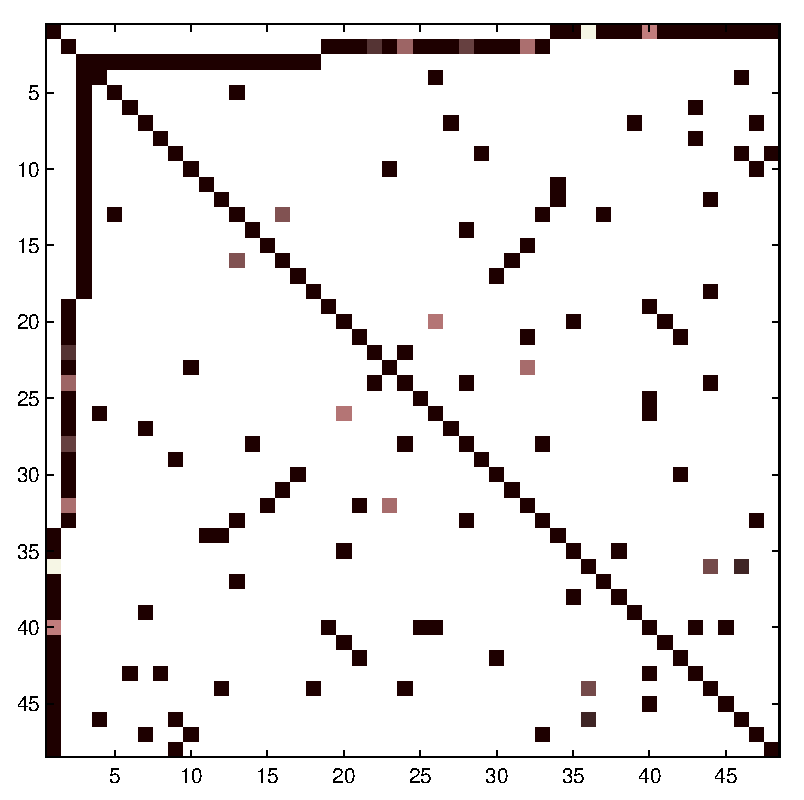
\includegraphics[width=3cm]{fig/disjoint_om}
%  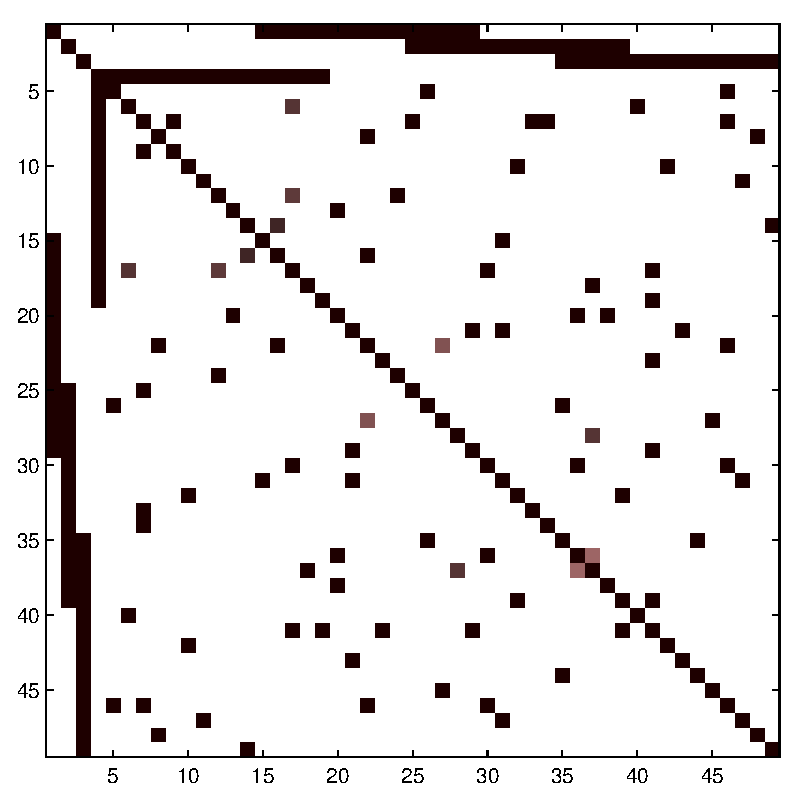
\includegraphics[width=3cm]{fig/overlap_om}
%  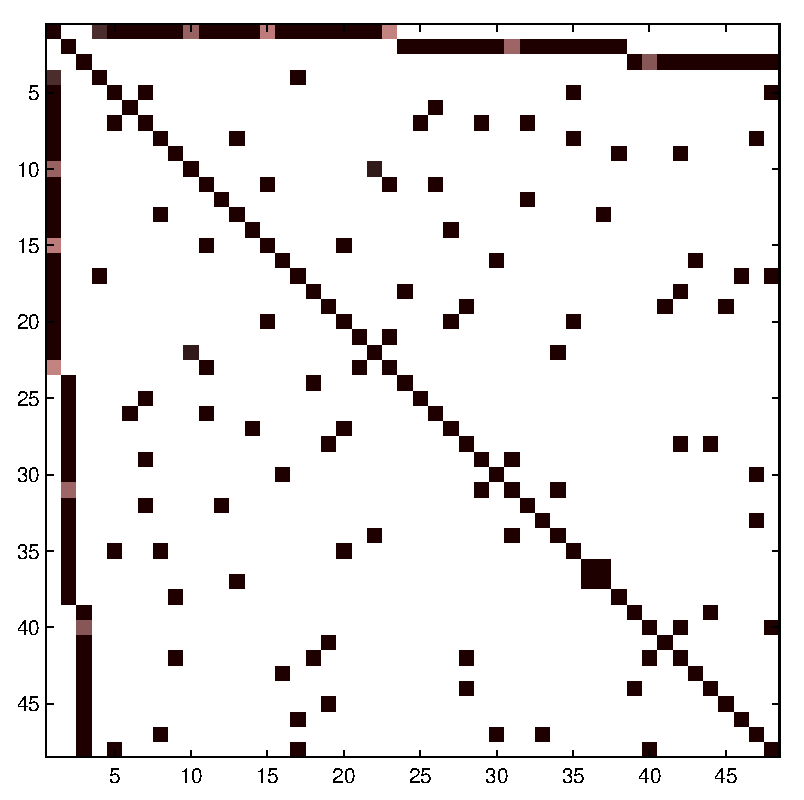
\includegraphics[width=3cm]{fig/diff_om}
%  \end{minipage}
%  \begin{minipage}[ccc]{\linewidth}
%  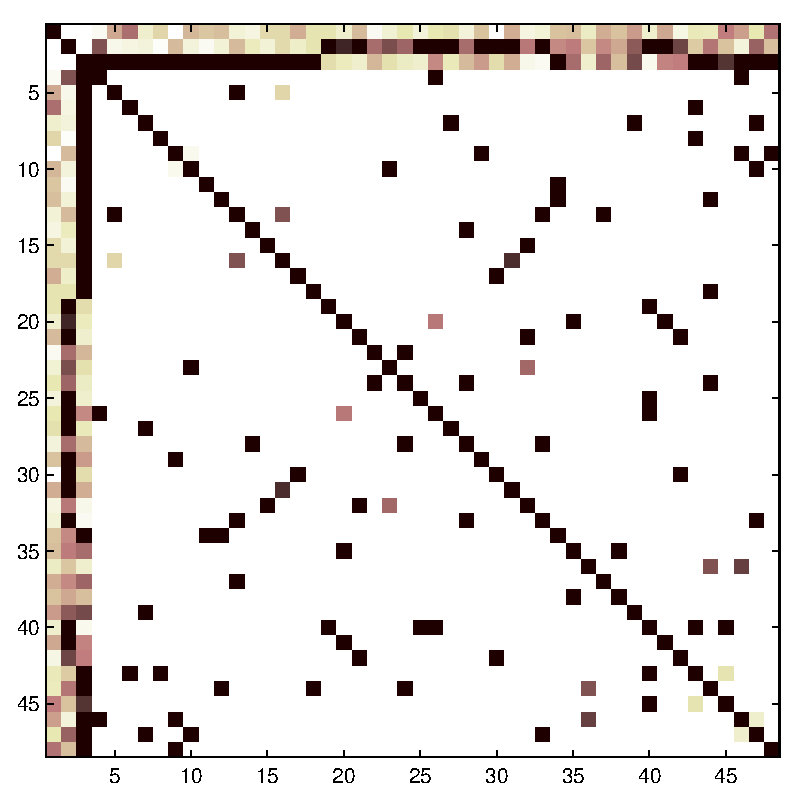
\includegraphics[width=3cm]{fig/disjoint_tr}
%  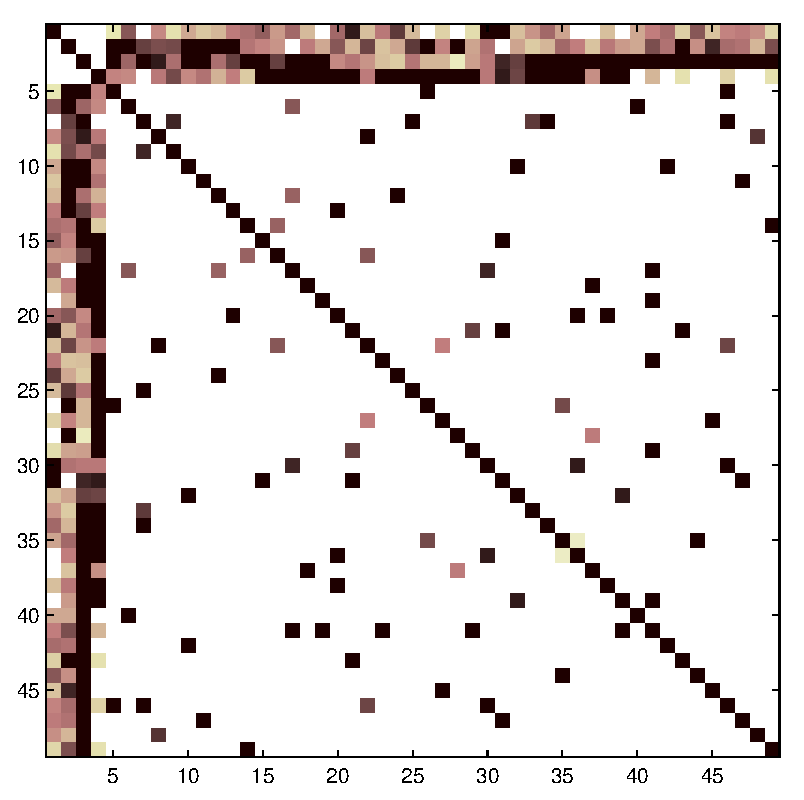
\includegraphics[width=3cm]{fig/overlap_tr}
%  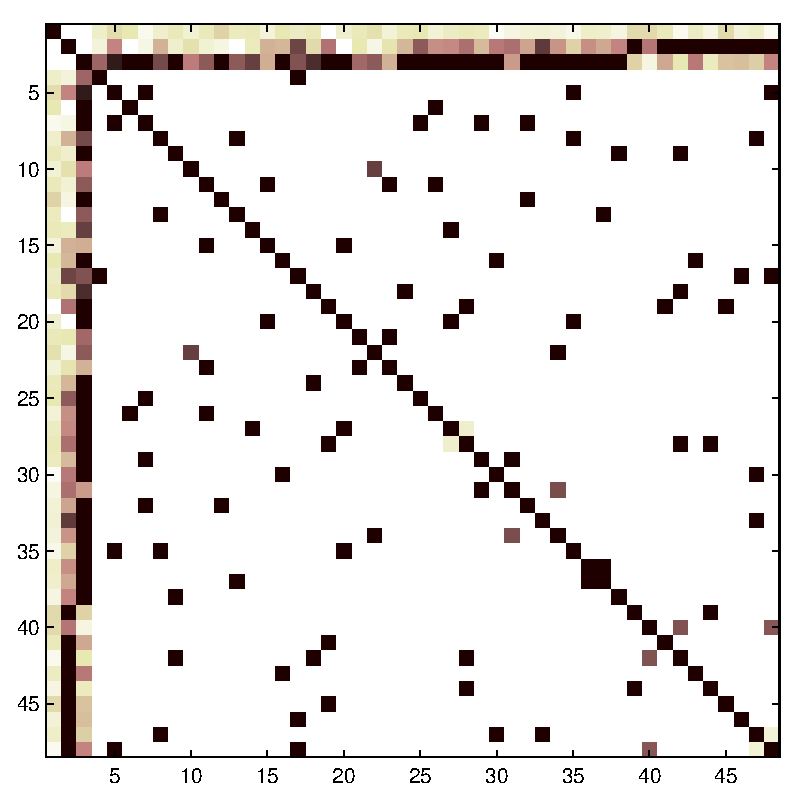
\includegraphics[width=3cm]{fig/diff_tr}
%  \end{minipage}
%  \caption{Experiment for the $k$-chain group Lasso. Top:number of pivots, i.e., drop/full step in active set. Left figure shows the number of pivots per active set call and right plot shows the total number of pivots during iterations. Bottom: evolution of the number of active atoms in our algorithm.}
%\end{figure}

%\begin{figure}
%\center
%\hfill
%\subfigure[Title A]{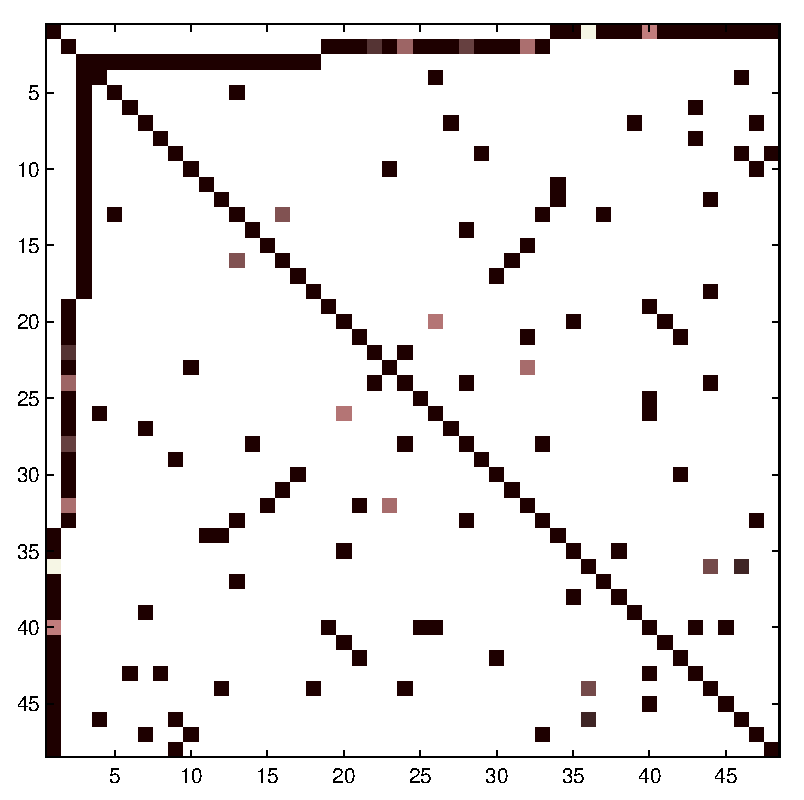
\includegraphics[width=3cm]{fig/disjoint_om}}
%\hfill
%\subfigure[Title B]{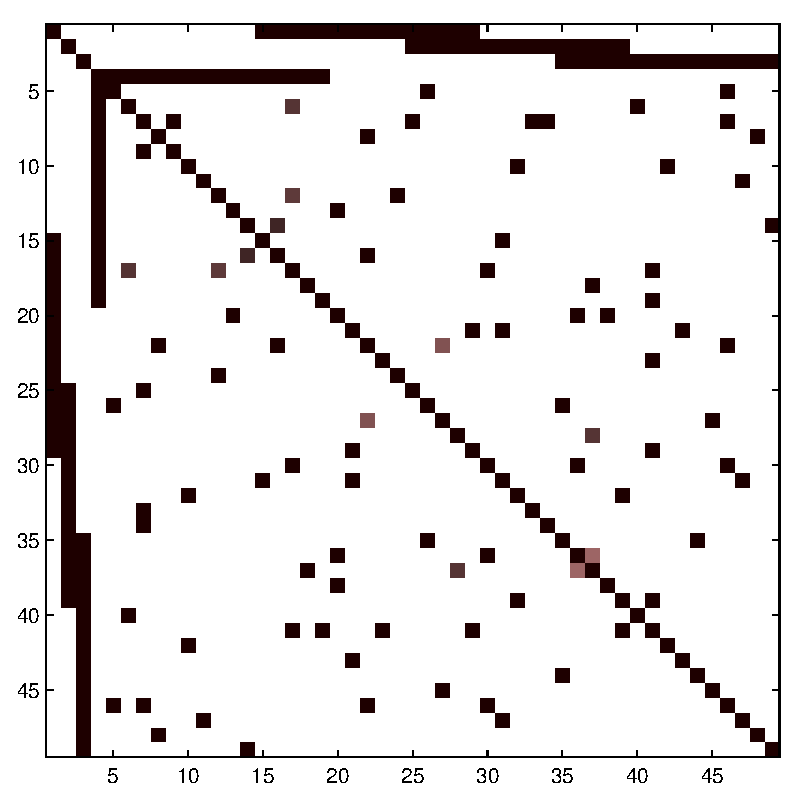
\includegraphics[width=3cm]{fig/overlap_om}}
%\hfill
%\subfigure[Title C]{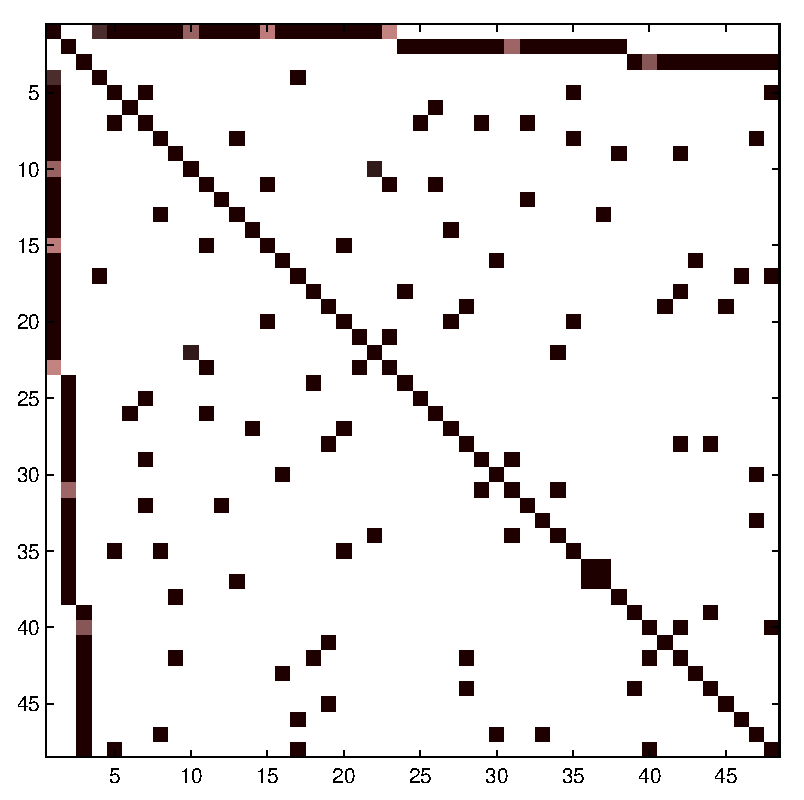
\includegraphics[width=3cm]{fig/diff_om}}
%\hfill
%\\
%\subfigure[Title A]{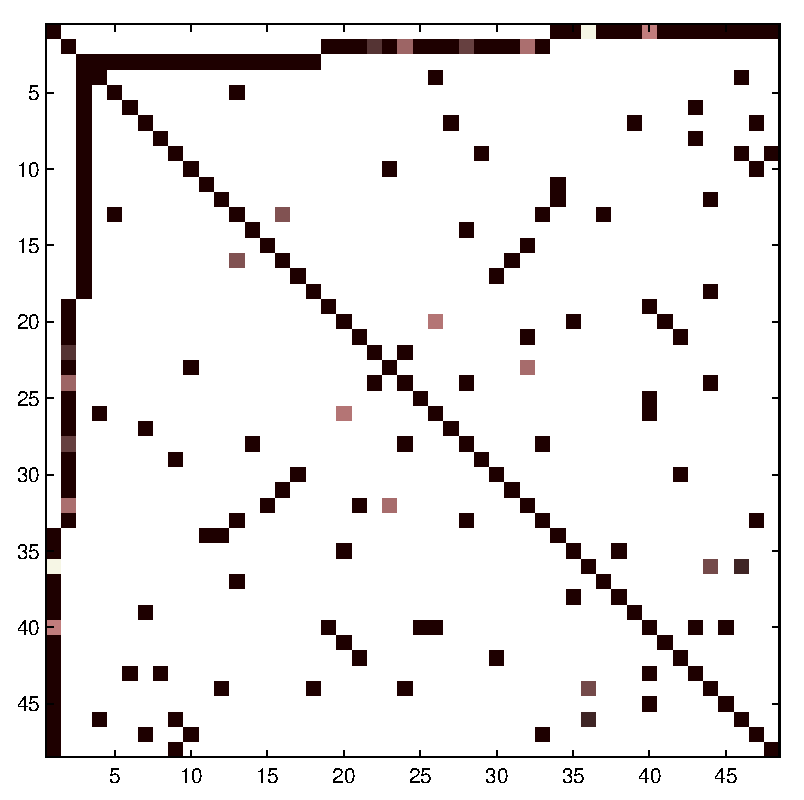
\includegraphics[width=3cm]{fig/disjoint_om}}
%\hfill
%\subfigure[Title B]{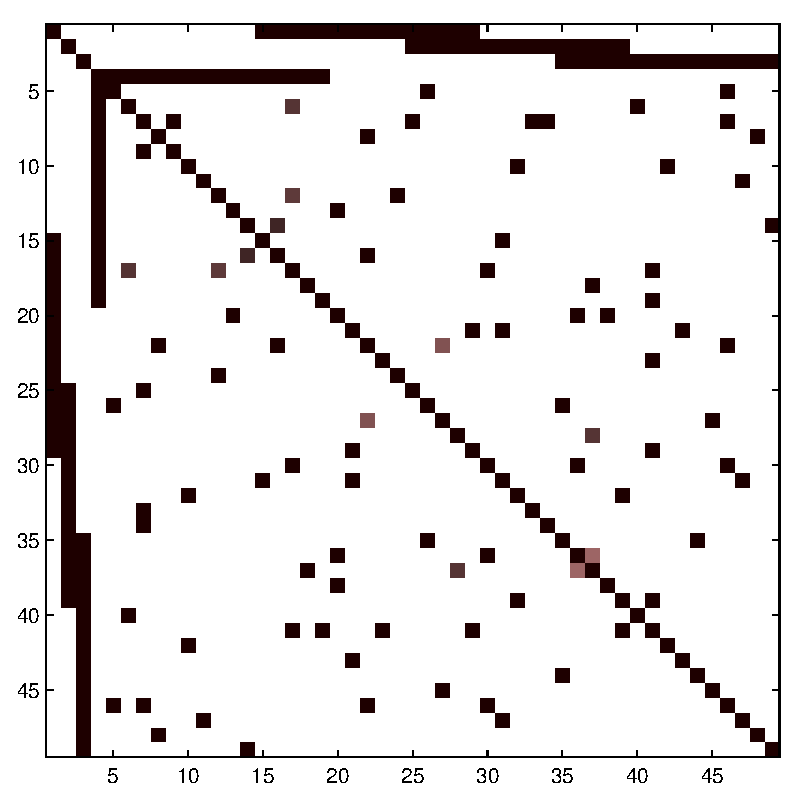
\includegraphics[width=3cm]{fig/overlap_om}}
%\hfill
%\subfigure[Title C]{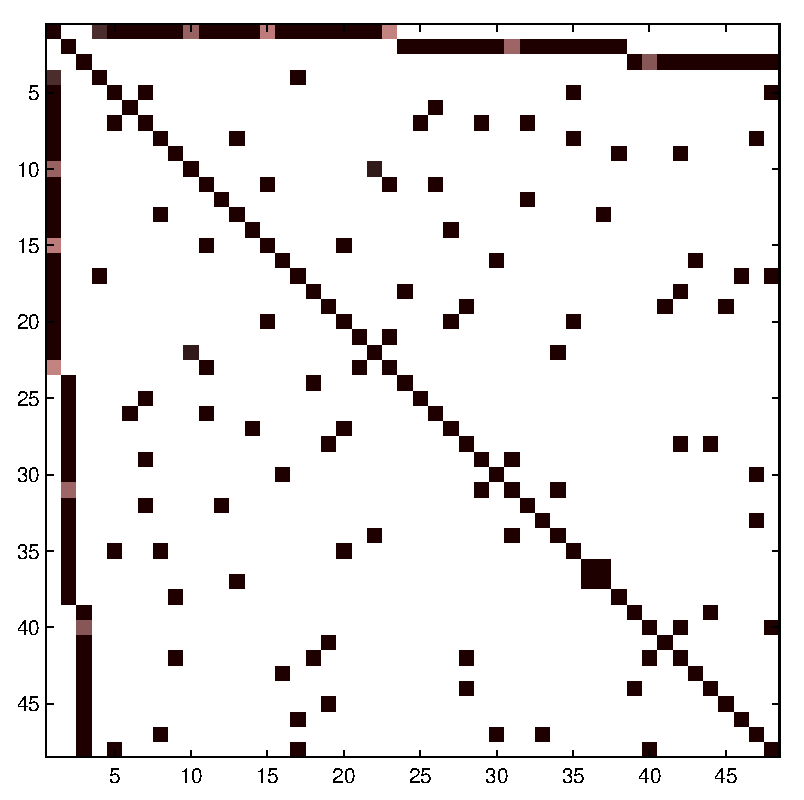
\includegraphics[width=3cm]{fig/diff_om}}
%\hfill
%\caption{Title for both}
%\end{figure}

%\begin{figure}
%\center
%\hfill
%\subfigure[Title A]{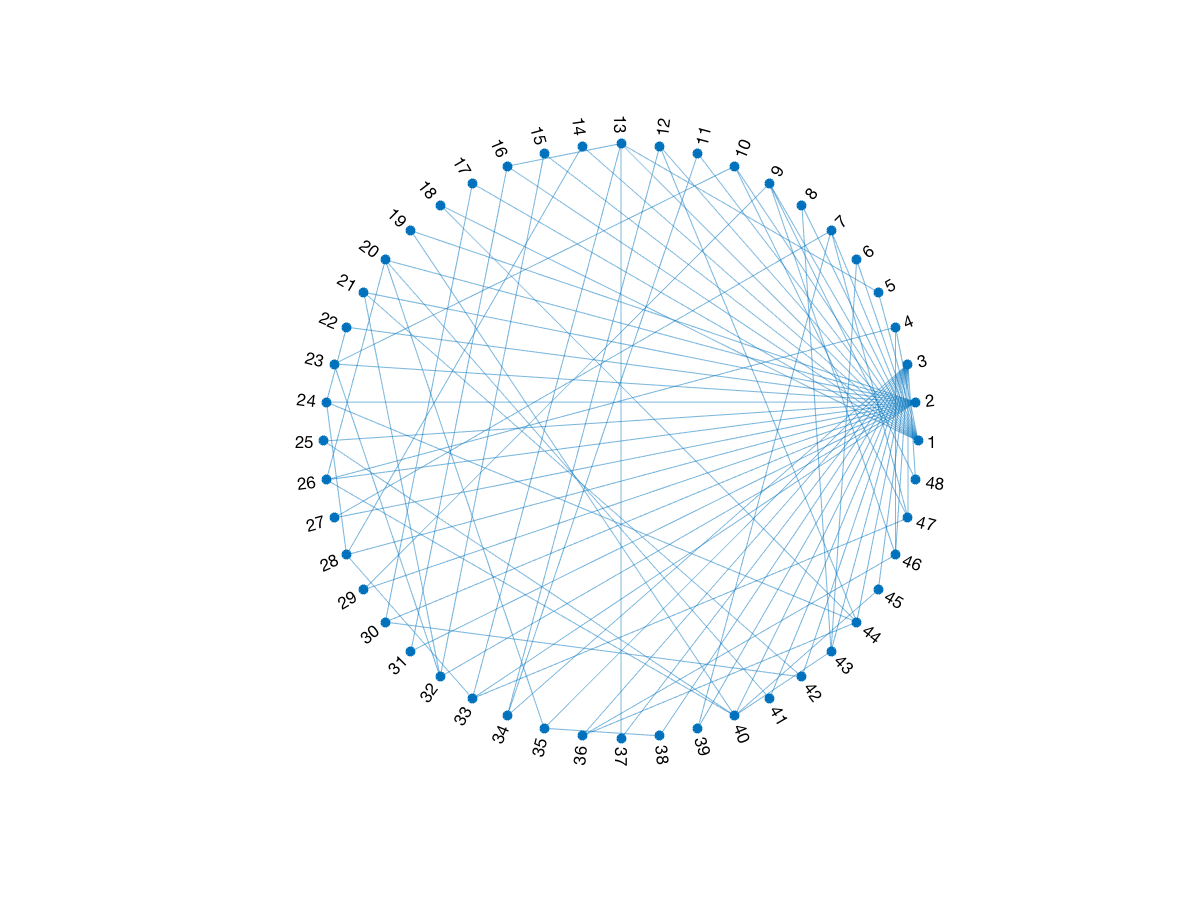
\includegraphics[width=4cm]{fig/disjoint_graph}}
%\hfill
%\subfigure[Title B]{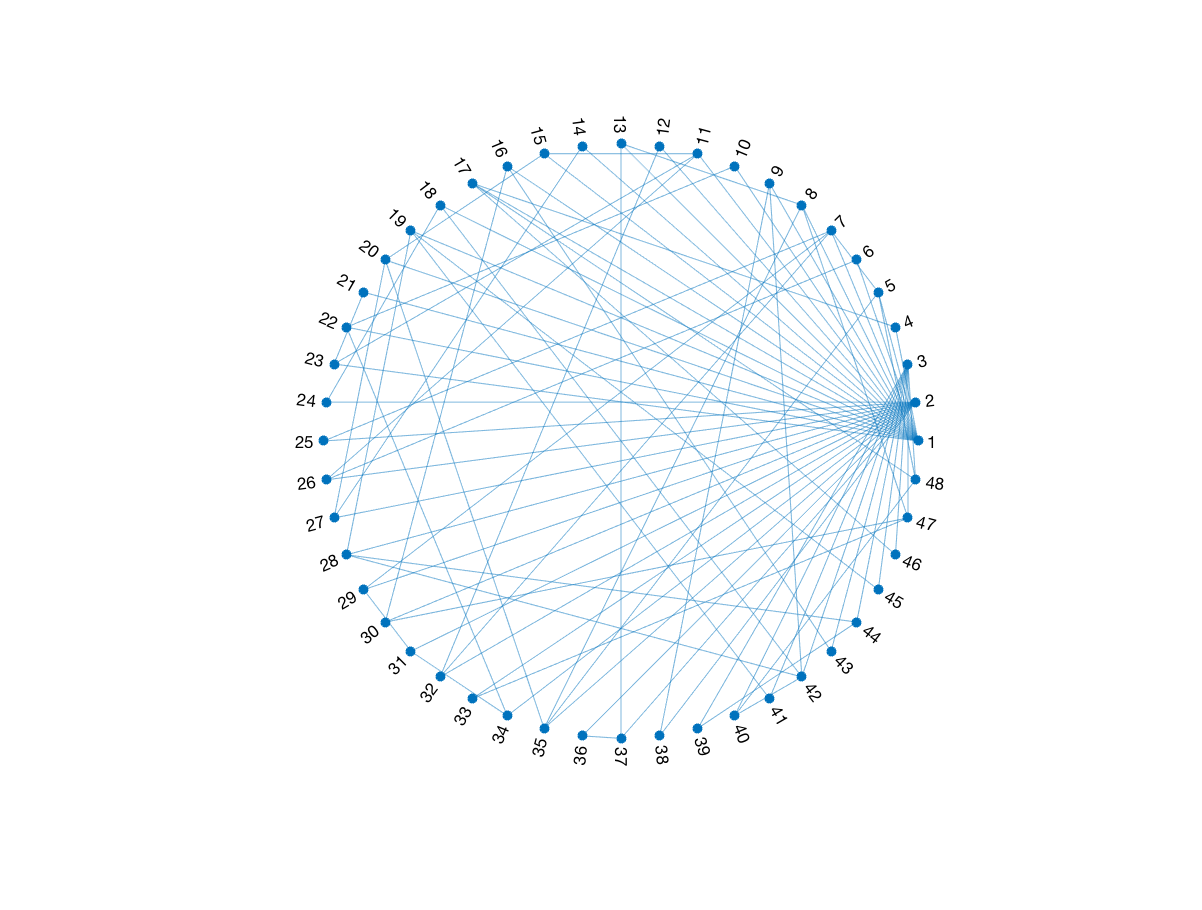
\includegraphics[width=4cm]{fig/diff_graph}}
%\hfill
%\subfigure[Title C]{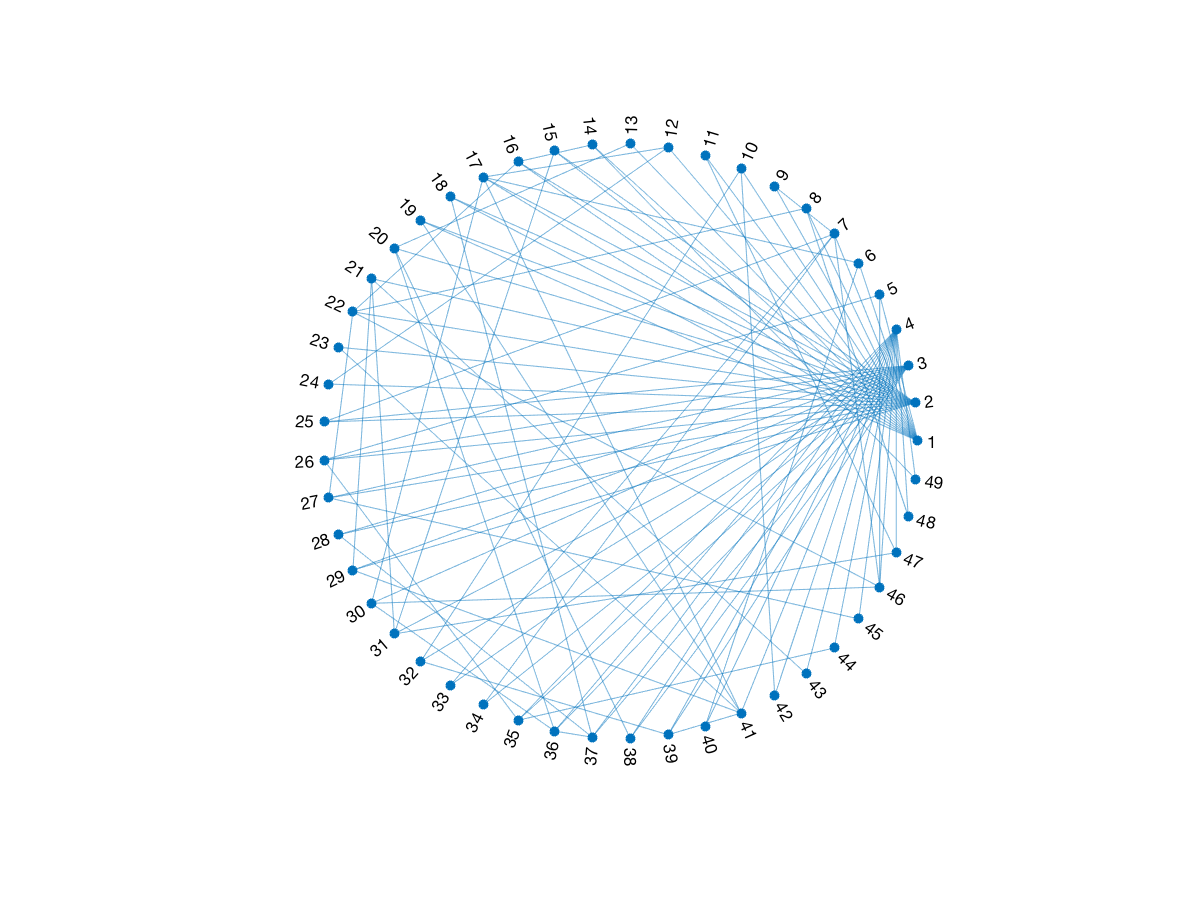
\includegraphics[width=4cm]{fig/over_graph}}
%\caption{Title for both}
%\end{figure}

%\begin{figure}
%\label{fig:synth}
%\center
%\hfill
%\subfigure[ours]{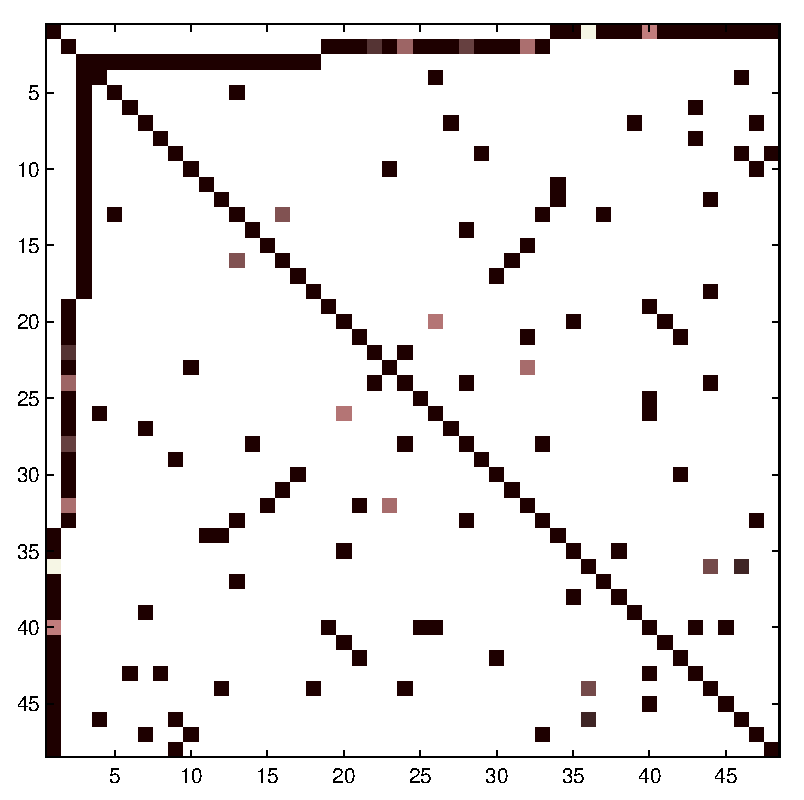
\includegraphics[width=2.2cm]{fig/disjoint_om}}
%\hfill
%\subfigure[$\ell_1+\tr$]{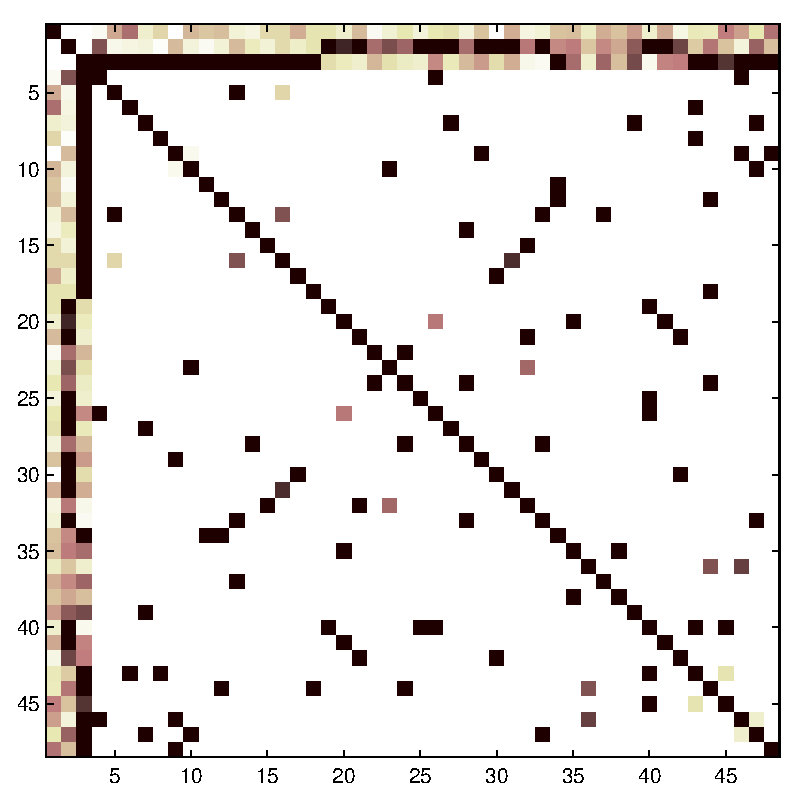
\includegraphics[width=2.2cm]{fig/disjoint_tr}}
%\hfill
%\subfigure[ours]{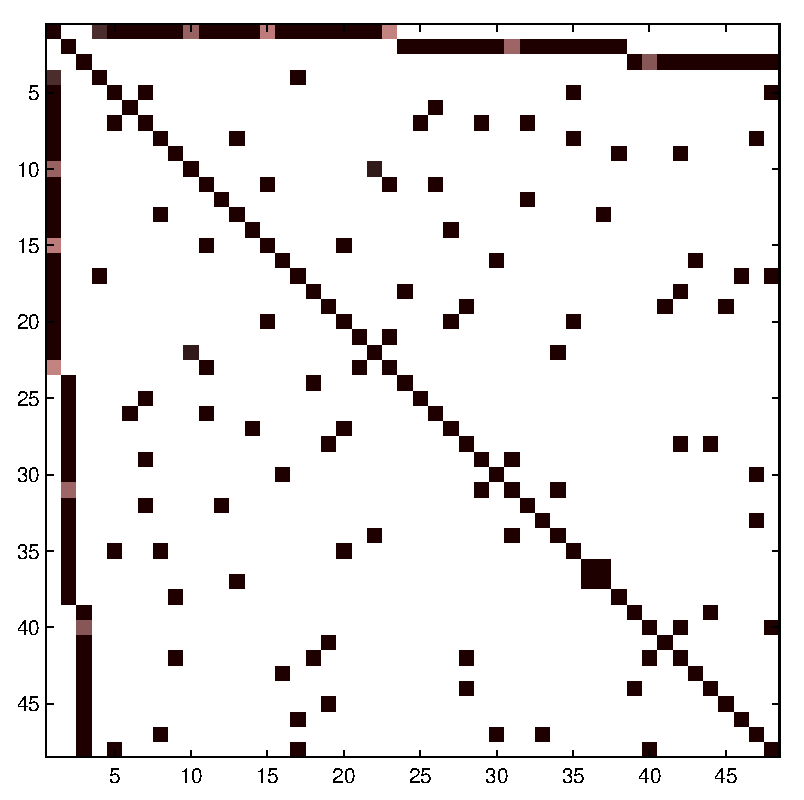
\includegraphics[width=2.2cm]{fig/diff_om}}
%\hfill
%\\
%\subfigure[$\ell_1+\tr$]{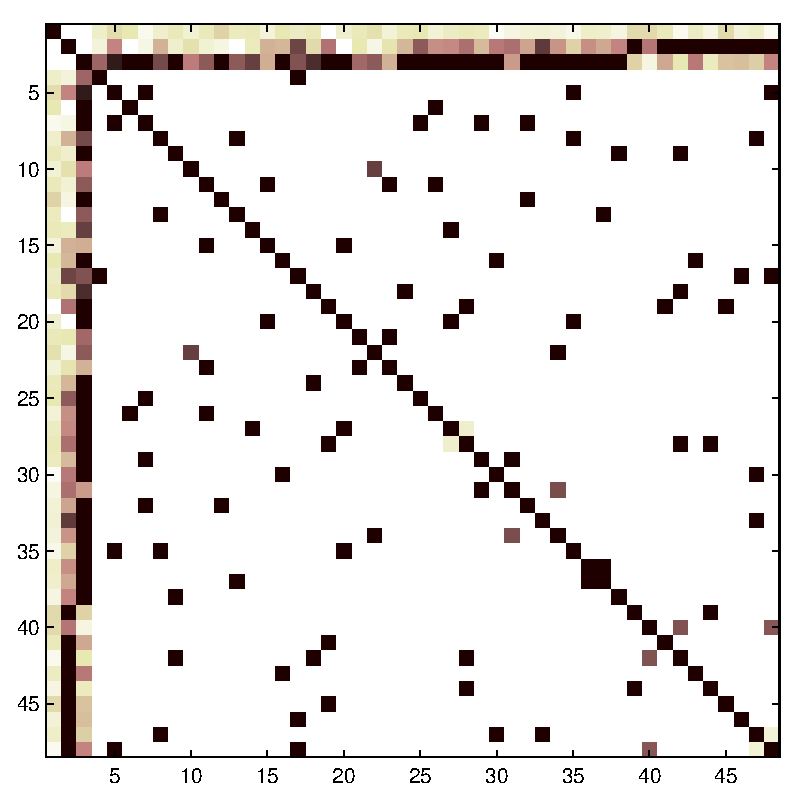
\includegraphics[width=2.2cm]{fig/diff_tr}}
%\hfill
%\subfigure[ours]{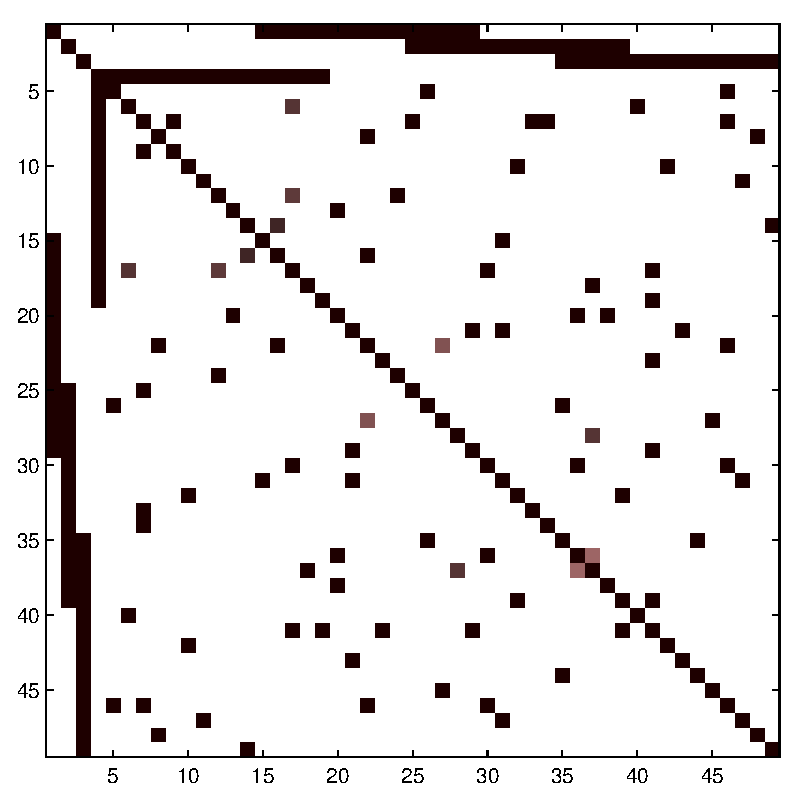
\includegraphics[width=2.2cm]{fig/overlap_om}}
%\hfill
%\subfigure[$\ell_1+\tr$]{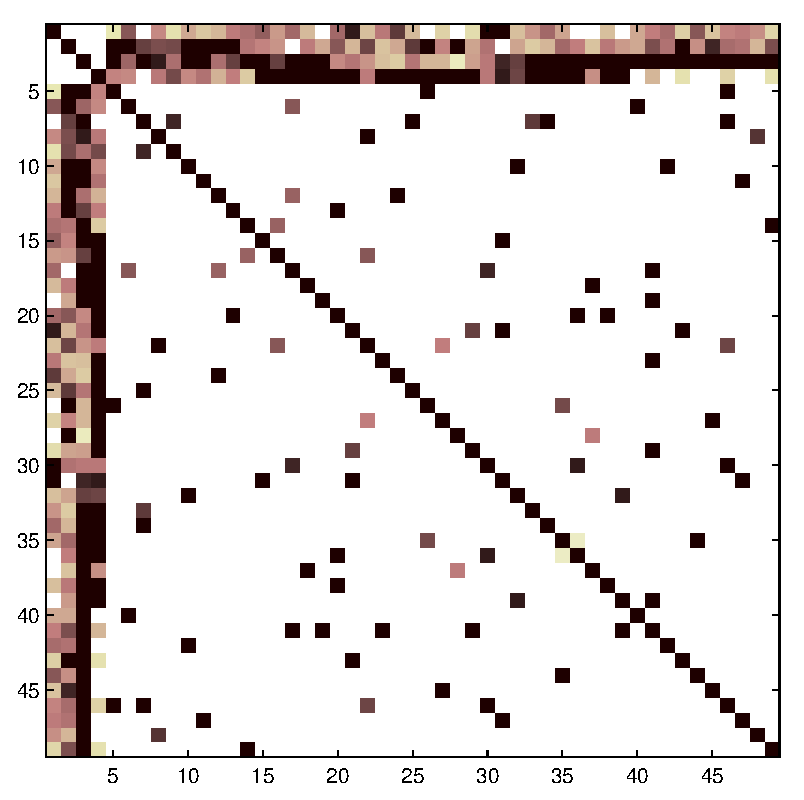
\includegraphics[width=2.2cm]{fig/overlap_tr}}
%\hfill
%\caption{Estimated complete concentration matrices: for \textit{model 1} in (a) ours and (b) $\ell_1+\tr$ regularization; for \textit{model 2} in (c) ours and (d) $\ell_1+\tr$ regularization; for \textit{model 3} in (e) ours and (f) $\ell_1+\tr$ regularization }
%\end{figure}



\begin{figure}
\label{fig:synth}
\center
\begin{tabular}{ccc}
  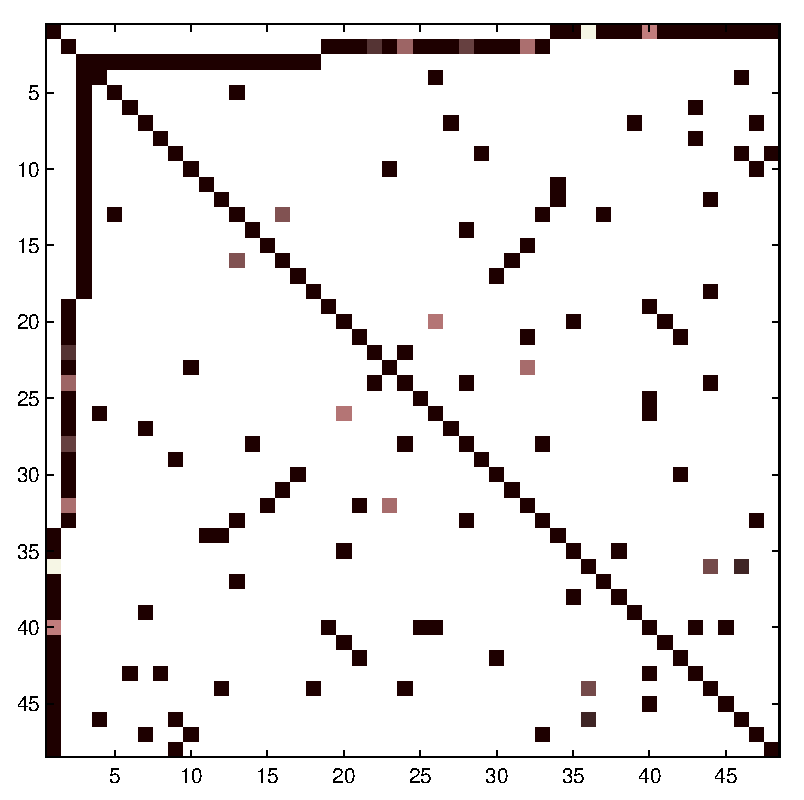
\includegraphics[width=3.5cm]{fig/disjoint_om} 
  &   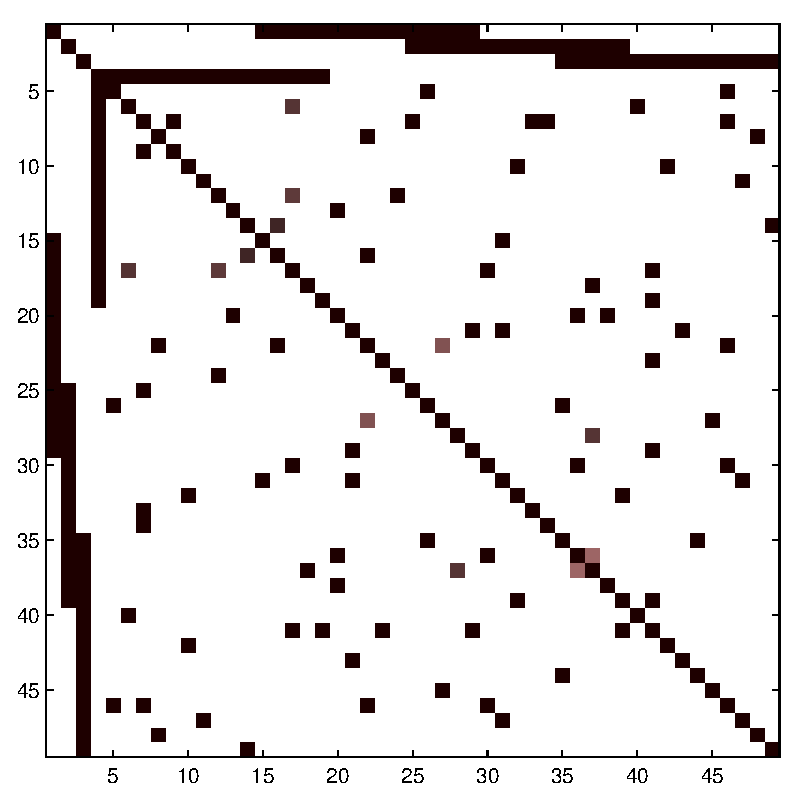
\includegraphics[width=3.5cm]{fig/overlap_om}
  &   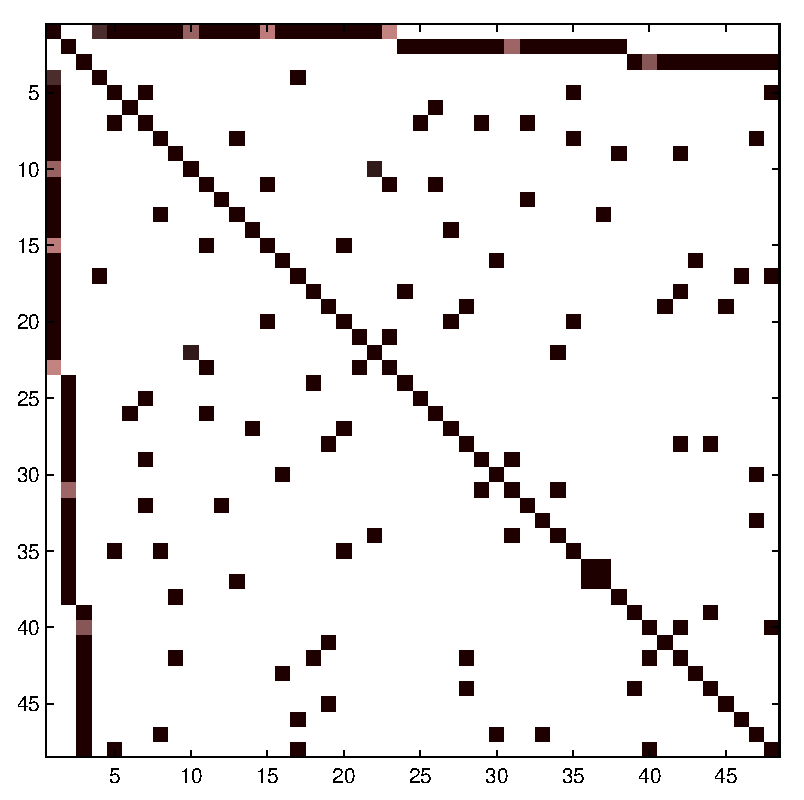
\includegraphics[width=3.5cm]{fig/diff_om}
   \\    (a) \textit{model 1}, ours & (b)  \textit{model 2}, ours  & (c)  \textit{model 3}, ours  \\[6pt]
 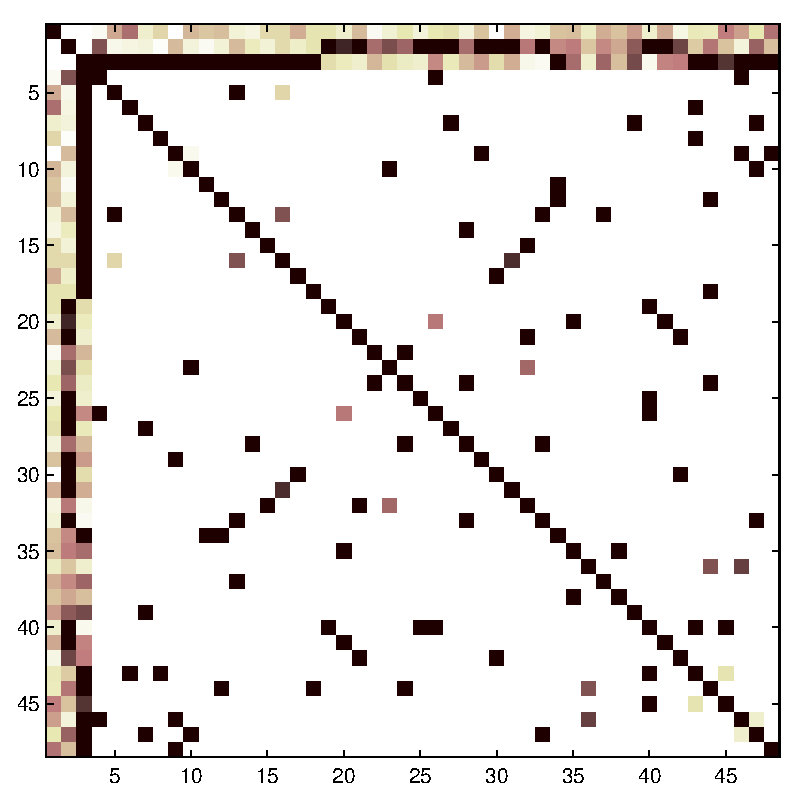
\includegraphics[width=3.5cm]{fig/disjoint_tr} 
  &   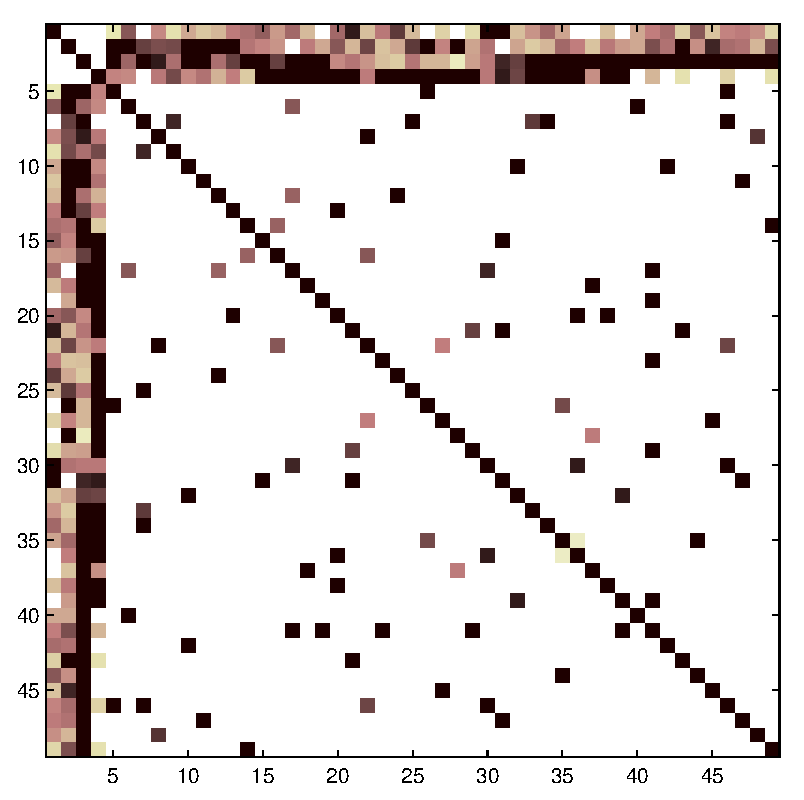
\includegraphics[width=3.5cm]{fig/overlap_tr}
  &   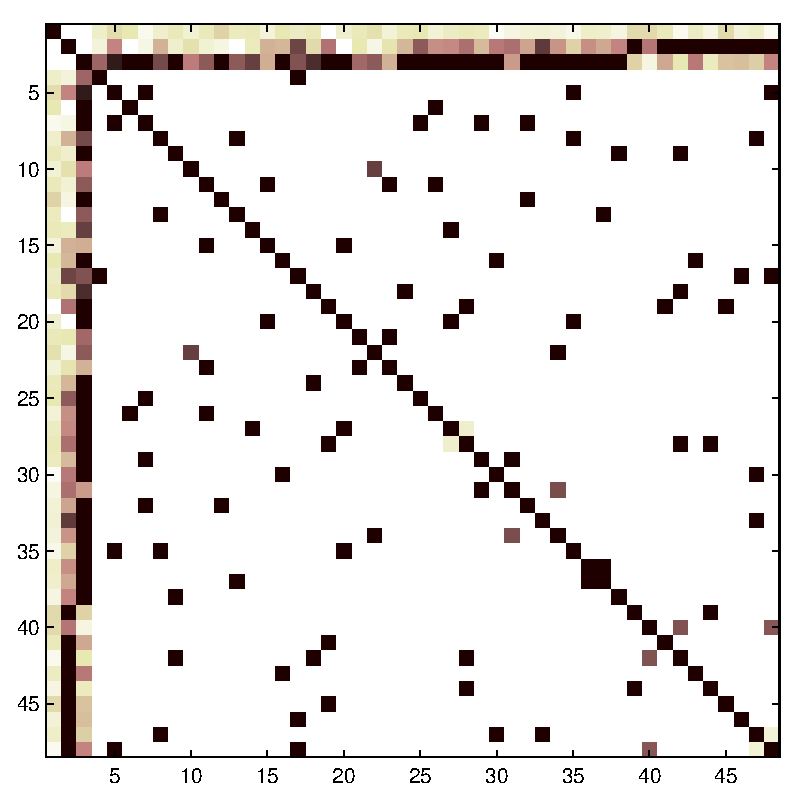
\includegraphics[width=3.5cm]{fig/diff_tr}
   \\    (d)  \textit{model 1}, $\ell_1+\tr$ & (e)  \textit{model 2}, $\ell_1+\tr$  & (f)  \textit{model 3}, $\ell_1+\tr$  \\[6pt]
\end{tabular}
\caption{Estimated $|K_{ij}|$, for $K$ the complete concentration matrices where the three (resp. four) first rows and columns correspond to the latent variables of \textit{model 1} and \textit{model 3} (resp. \textit{model 2}) : for \textit{model 1} in (a) ours and (d) $\ell_1+\tr$ regularization; for \textit{model 2} in (b) ours and (e) $\ell_1+\tr$ regularization; for \textit{model 3} in (c) ours and (f) $\ell_1+\tr$ regularization }
\end{figure}


\subsection{Microarray dataset}

We consider the MILE data \citep{haferlach2010clinical} that measure the mRNA expression levels of 16,853 genes in 541 patients with acute myeloid leukemia (AML), an aggressive blood cancer. The activity of genes is coupled by the activation of biological pathways. This motivates to search for a graphical model with latent variables connected to blocks of genes.

We selected 250 genes with higher variance. We fix the size of the blocks to $k=100$ for our method and compare with the regularized maximum log-likelihood formulation of \citet{chandrasekaran2010}. The obtained empirical covariance matrix has very concentrate eigenvalues and the two first eigenvectors capture most of the covariance. Thus we select parameters for \citet{chandrasekaran2010} such as to recover a low rank component $\hat{L}_{tr}$ of rank two and sparse comonent $\hat{S}_{tr}$  . We then select the parameters of our method such as : to recover a sparse component with comparable level of sparsity as $\hat{S}_{tr}$ (cf. appendix), and a sparse low rank component  $\hat{L}_ours$. Figure \ref{fig:gen} shows qualitative results. (a) shows $\hat{S}_{tr}$; (b) shows the low rank sparse component $UU^{\top}$ recovered by our method. For a better visualization of the blocks we have reorered the lines of $U$ such that we group the genes belonging to the same groups. (c) shows $\hat{L}_{ours}$ and (d) shows $\hat{L}_{tr}$ with same order. \citet{chandrasekaran2010} does not recover the block structure while our method provides dense blocks.
%Both methods recover similar block of genes but our method provides more
%and  also genes highly associated with AML: FLT3, NPM1, CEBPA, KIT, N-RAS, MLL, WT1. We fix the size of the blocks to $k=100$ for our method and compare with the regularized maximum log-likelihood. Parameters are chosen so that the two methods recover similar sparse components. Figure \ref{fig:gen} shows qualitative results. (a) shows the low rank sparse component $UU^{\top}$ recovered by our method and (b) is the support of $U$. For a better visualization of the blocks we have reorered the lines of $U$ using Gray code. (c) shows the low rank component estimated by the the regularized maximum log-likelihood and (d) shows this same component reordered according to the blocks found by our method. Both methods seem to recover similar block of genes but our method provides more interpretability.

\begin{figure}
\label{fig:gen}
\center
\begin{tabular}{ccccc}
      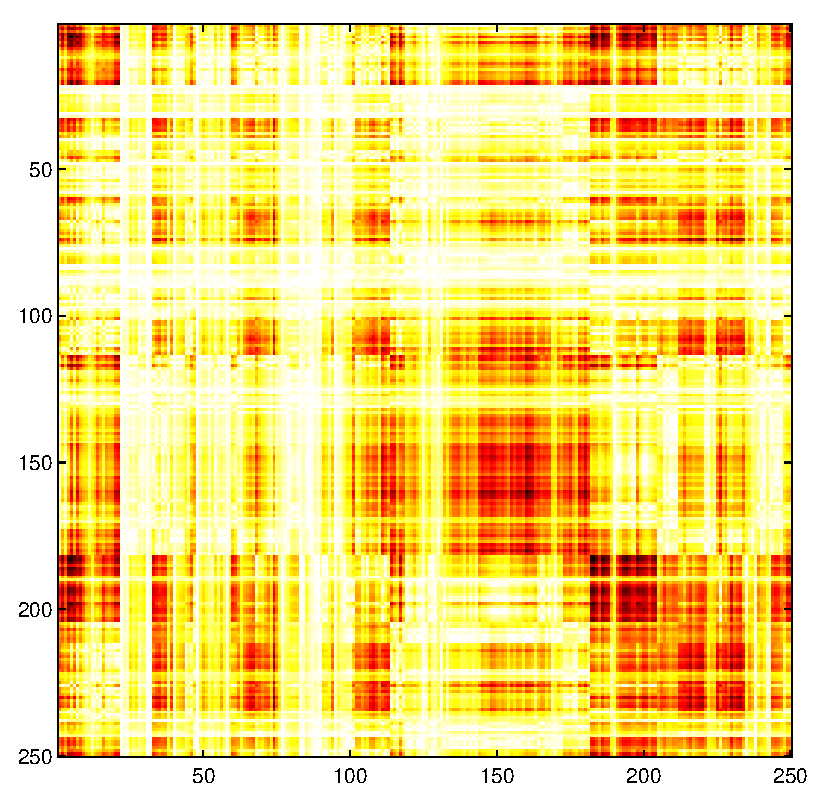
\includegraphics[width=4cm]{fig/MILE_Lsl_not_ordered}
  &   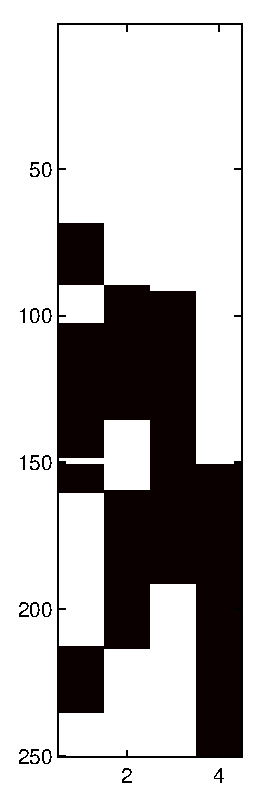
\includegraphics[height=3.8cm]{fig/MILE_blocks}
  &   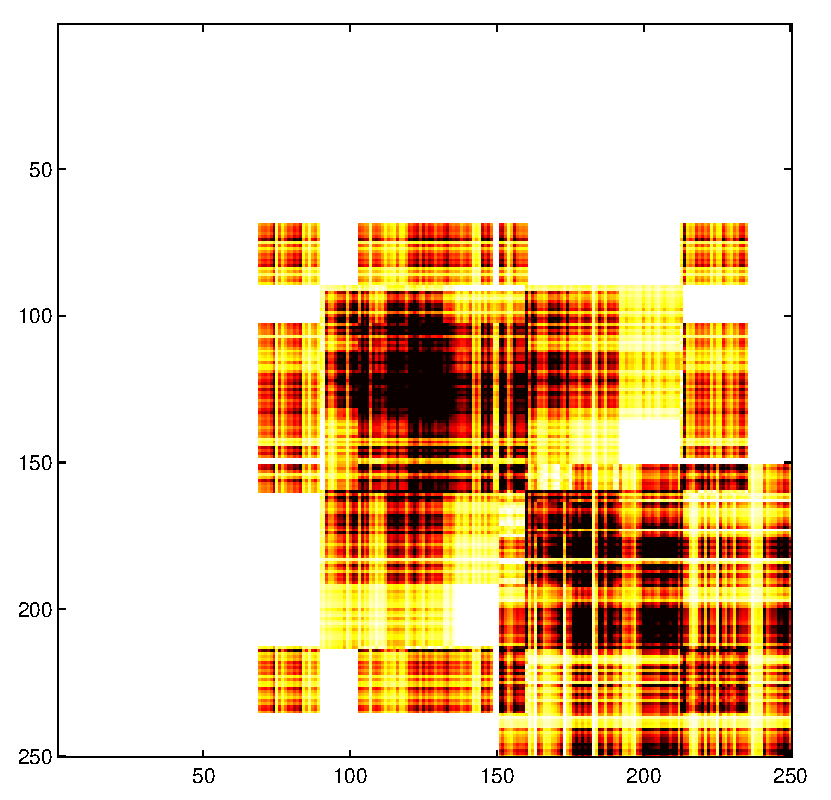
\includegraphics[width=4cm]{fig/MILE_Lom} 
  &   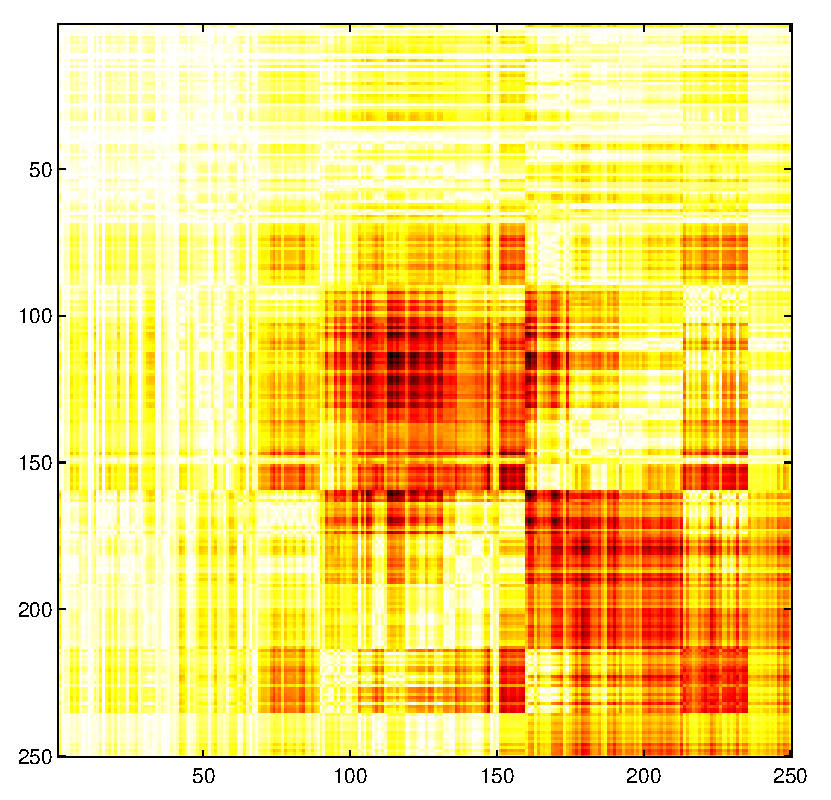
\includegraphics[width=4cm]{fig/MILE_Lsl_ordered} 
  &   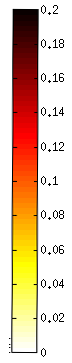
\includegraphics[height=3.8cm]{fig/colorbar} 
   \\   (a)  $\hat{L}_{tr}$  & (b) blocks &(c) $\hat{L}_{ours}$ &(d) $\hat{L}_{tr}$ ordered  
\end{tabular}
\caption{Estimated low rank component $\hat{L}_{tr}$ for \citet{chandrasekaran2010} (a);  the support of the 4 rank-one 100-sparse components $uu^{\top}$ for our estimated low rank component  (b);  our estimated low rank component (d); and $\hat{L}_{tr}$  with the same order as ours }
\end{figure}


\subsection*{Conclusion}
We consider a family of latent variable Gaussian graphical model whose concentration matrix has a sparse plus low-rank structure. We introduce a regularization to impose more structure on the low rank component, as a sum of multiple low-rank and $k$-sparse factors, and derive a convex formulation. We propose an efficient algorithm to optimize this problem and show promising results for recovering the structure of the complete GGM in the experiments. We provide a first result for identifiability condition. Futurework includes extending the framework to multiple levels of sparsity and generalizing identifiability conditions for recovery guarantees on our optimisation problem .


%\section*{References}
\bibliographystyle{apalike}
\bibliography{lvggm}

\end{document}
